% id: 0485
% book: RPM 중3-2 수학 · 04 원주각
% section: 유형 19 접선과 현이 이루는 각의 활용 – 한 점에서 원에 그은 두 접선
% figure: crop:fig-0485.png
% answer: $67^\circ$
% answer_source: 답지
% variant_level: 0 (원본 전사)
% 이 파일은 build.mjs 가 items.json 에서 만든다. 고칠 때는 items.json 을 고친다.
\smash{\raisebox{1.5mm}{\dmkichul{대표문제}}}
\noindent\begin{minipage}[t]{0.58\linewidth}\vspace{0pt}\raggedright 오른쪽 그림에서 원~$\pt{O}$는 $\triangle\pt{ABC}$의 내접원이면서 $\triangle\pt{DEF}$의 외접원이다. $\angle\pt{DBE}=50^\circ$, $\angle\pt{DEF}=48^\circ$일 때, $\angle\pt{EDF}$의 크기를 구하시오.\end{minipage}\hfill\begin{minipage}[t]{0.4\linewidth}\vspace{0pt}\centering \setlength{\dmfigw}{98.2pt}\ifdim\dmfigw>\linewidth\setlength{\dmfigw}{\linewidth}\fi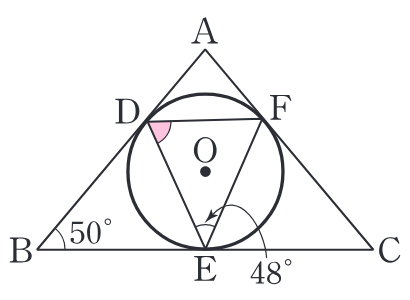
\includegraphics[width=\dmfigw]{figures/fig-0485.png}\end{minipage}\par
